\section{Algebraic Moment Closures}
\label{sec:algebraicClosure}

Algebraic moment closures for the two-moment model are computationally efficient as they provide the Eddington factor in Eq.~\eqref{eq:eddingtonTensor} in closed form as a function of the density $\cJ$ and the flux factor $h=|\vect{\cH}|/\cJ$.  
The family of algebraic closures we consider in this paper can be written in the form \cite{cernohorskyBludman_1994}
\begin{equation}
  \chi(\cJ,h)=\f{1}{3}+\f{2\,(1-\cJ)\,(1-2\cJ)}{3}\,\Theta\Big(\f{h}{1-\cJ}\Big),
  \label{eq:eddingtonFactor}
\end{equation}
where the closure function $\Theta(x)$ varies with the specifics of the closure procedure.  
We will consider two basic closure procedures in more detail below: the maximum entropy (ME) closure and the Kershaw (K) closure.  

\paragraph{Low Occupancy Limit}
We note in passing that in the low occupancy limit ($\cJ\ll1$), the Eddington factor in Eq.~\eqref{eq:eddingtonFactor} becomes independent of $\cJ$; i.e.,
\begin{equation}
  \chi(\cJ,h)\to\chi_{0}(h)=\f{1}{3}+\f{2}{3}\,\Theta\big(h\big).  
  \label{eq:eddingtonFactorLow}
\end{equation}

\subsection{Maximum Entropy Closure}

The basic principle behind the maximum entropy closure is that one can approximate the real fermion distribution with a distribution which have the Fermi-Dirac distribution form 
\begin{equation}
f(\omega)=\f{1}{e^{a + b\omega}+1}, 
\end{equation} 
meanwhile maximize the entropy function
\begin{equation}
S[f(\omega)] = (1-f)\log(1-f) + f\log f.
\end{equation} 
Given moments $\cJ$ and $\vect{\cH}$, a distribution satisfying above requirements can be found. 
Therefore, the stress tensor $\vect{\cK}$.

One ME closure given by Chernohorsky \& Bludman \cite{cernohorskyBludman_1994} is
\begin{equation}
  \Theta_{\mbox{\tiny ME}}^{\mbox{\tiny CB}}(x)
  =x^{2}\,\big(\,3-x+3\,x^{2}\,\big).
\end{equation}

Another ME closure given by Banach \& Larecki \cite{banachLarecki_2017b} is
\begin{equation}
  \Theta_{\mbox{\tiny ME}}^{\mbox{\tiny BL}}(x)
  =\f{1}{8}\,\big(\,9\,x^{2}-5+\sqrt{33\,x^{4}-42\,x^{2}+25}\,\big).
\end{equation}

\subsection{Kershaw Closure}
The basic principle behind Kershaw closure is derived from the fact that $\cR$ is convex.
Due to the convexity, one can write any element in $\cR$ as a convex combination of the elements on the realization boundary. 
Therefore, Kershaw closure satisfies realizability inherently.
For fermionic radiation, the boundary is based on the Heaviside step functions.
Here we introduce a closure function $\Theta(x)$ given by Banach \& Larecki \cite{banachLarecki_2017a}:
\begin{equation}
  \Theta_{\mbox{\tiny K}}^{\mbox{\tiny BL}}(x)=x^{2}
\end{equation}

Figure~\ref{fig:MabWithDifferentClosure} illustrates the behavior of these four closure.
As it shows, Minerbo closure (right bottom) is the only one among those four closures that does not preserve realizability.
\begin{figure}[h]
  \centering
  \begin{tabular}{cc}
    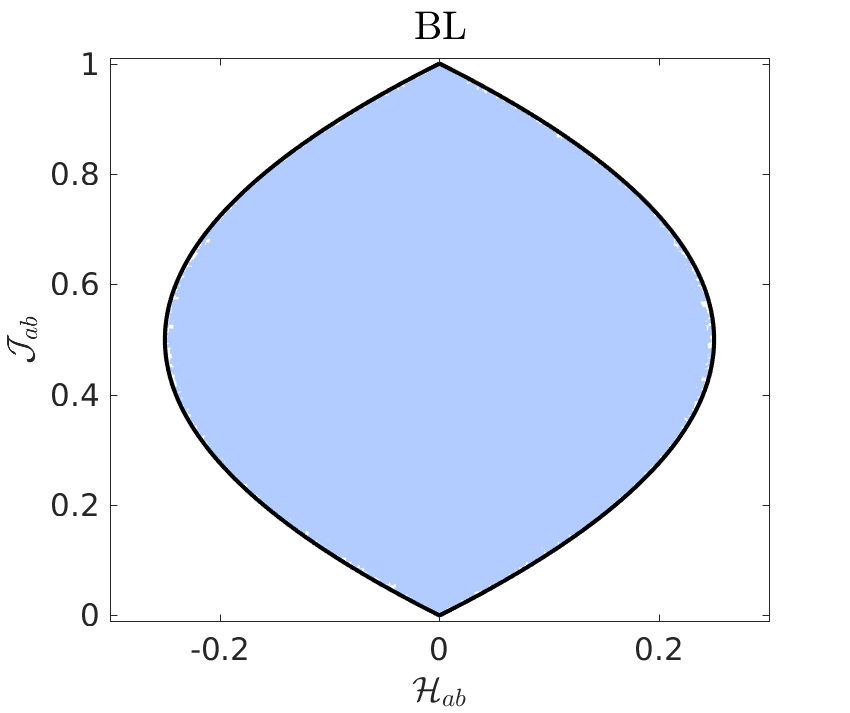
\includegraphics[width=0.5\textwidth]{figures/MabWithBLME}
    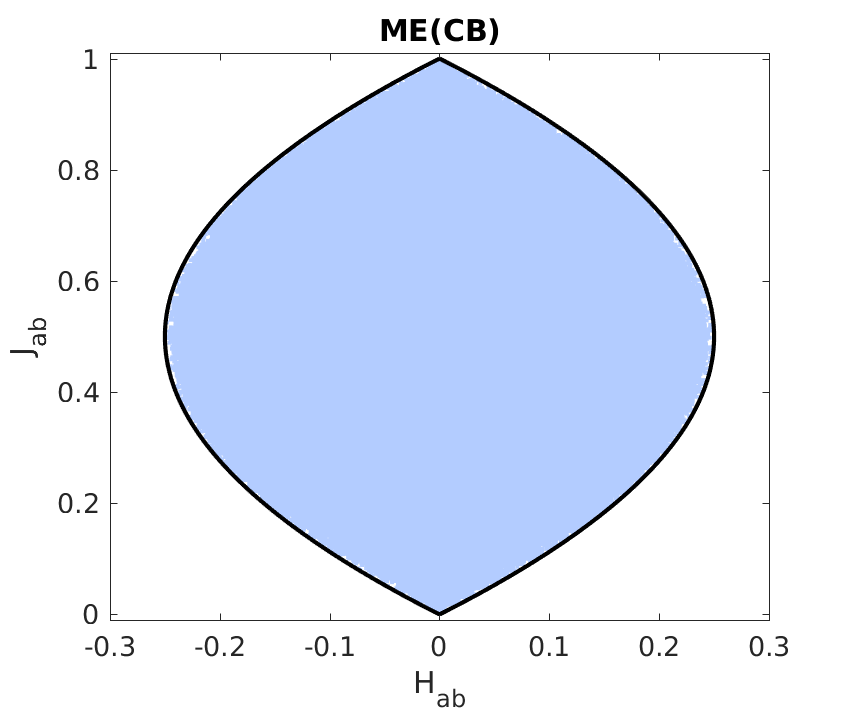
\includegraphics[width=0.5\textwidth]{figures/MabWithCBME} \\
    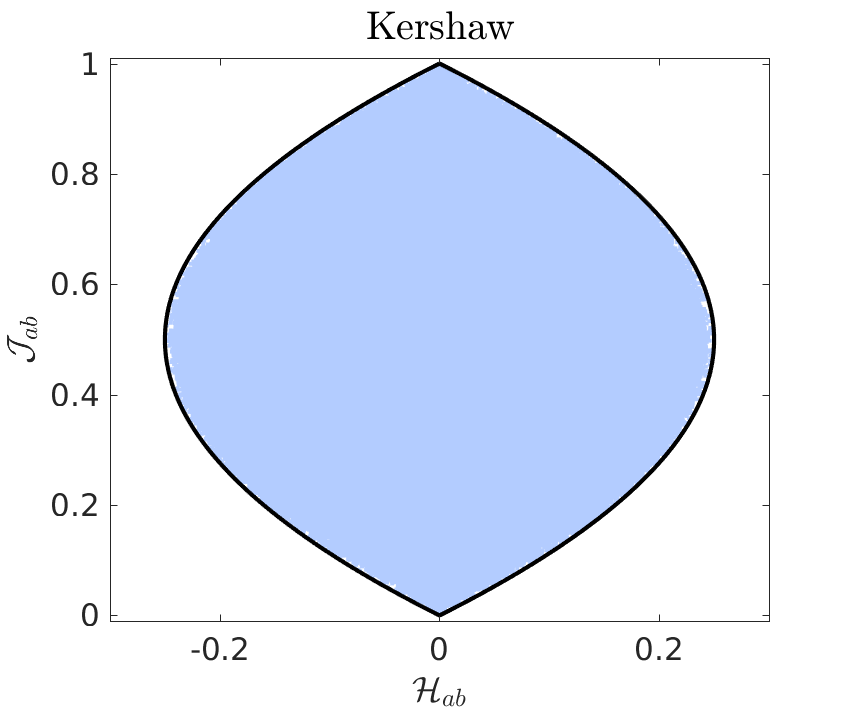
\includegraphics[width=0.5\textwidth]{figures/MabWithBLKS}
    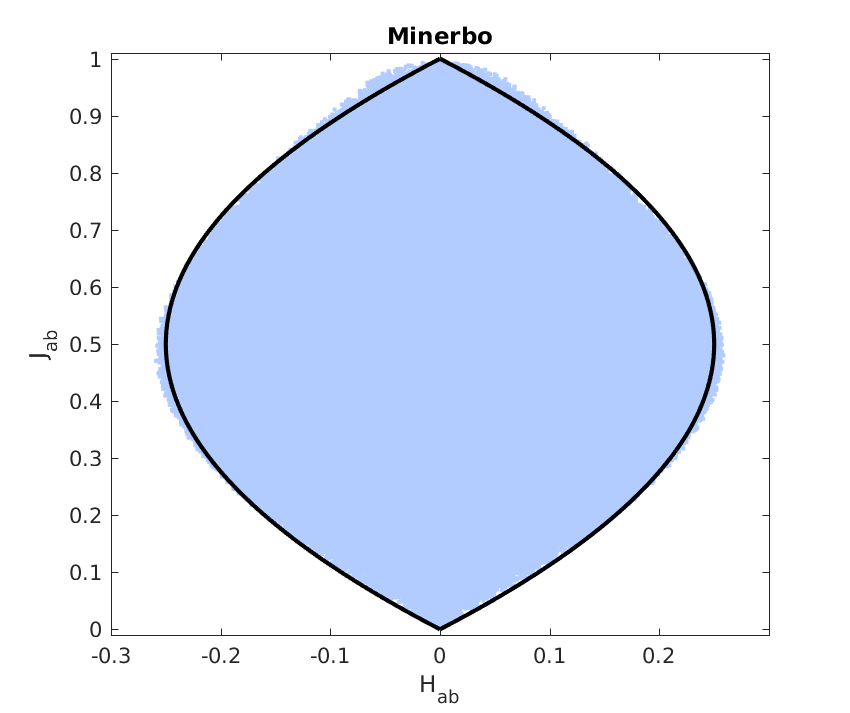
\includegraphics[width=0.5\textwidth]{figures/MabWithMI}
  \end{tabular}
   \caption{Illustration of $\vect{\cM}_{ab}$ with four different closures: Banach \& Larecki maximum entropy closure (left top), Chernohorsky \& Bludman maximum entropy closure (right top), Kershaw closure (left bottom), and Minerbo closure (right bottom).
   Total $10^{6}$ pairs of random Fermi-Dirac distribution were generated.
   With these pairs, $\vect{\cM}_{ab}$ with different closures were calculated separately and marked with light-blue points.
   Black lines define the boundary of $\cR$: $\gamma(\vect{\cM}) = 0$.}
  \label{fig:MabWithDifferentClosure}
\end{figure}